\pagebreak
\section{Vista Lógica} \label{vistaLogica}
La Vista Lógica muestra la estructura estática del sistema. En esta vista se representa la funcionalidad que el sistema proporcionará a los usuarios finales, es decir, se representa lo que el sistema debe hacer y las funciones y servicios que ofrece. Para esta vista se desarrollaron el Modelo Conceptual (ver Figura \ref{fig:diagrama_conceptual}) y el Modelo Entidad-Relación de la Base de Datos de la aplicación (ver Figura \ref{fig:er}). 

\begin{figure}[H]
   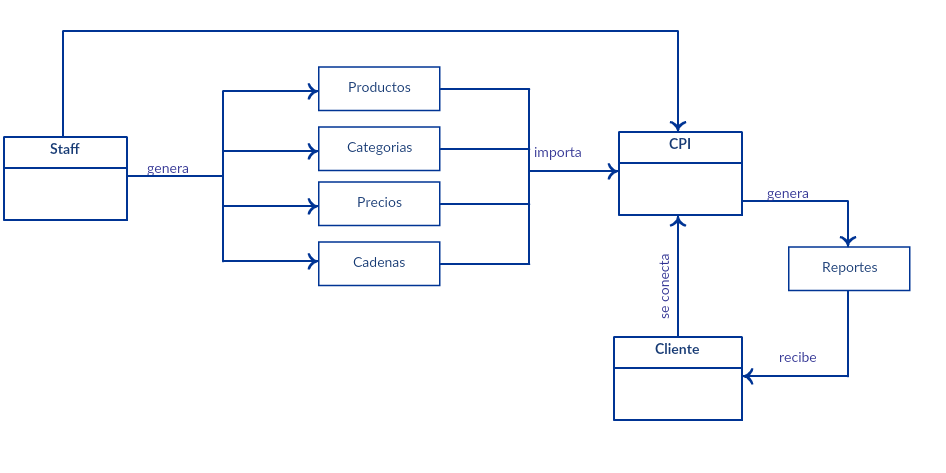
\includegraphics[width=\textwidth]{diagrama_conceptual.png}
   \caption{Modelo de Dominio. Elaboración propia.}
   \label{fig:diagrama_conceptual}
   \centering
\end{figure}

\begin{figure}[H]
       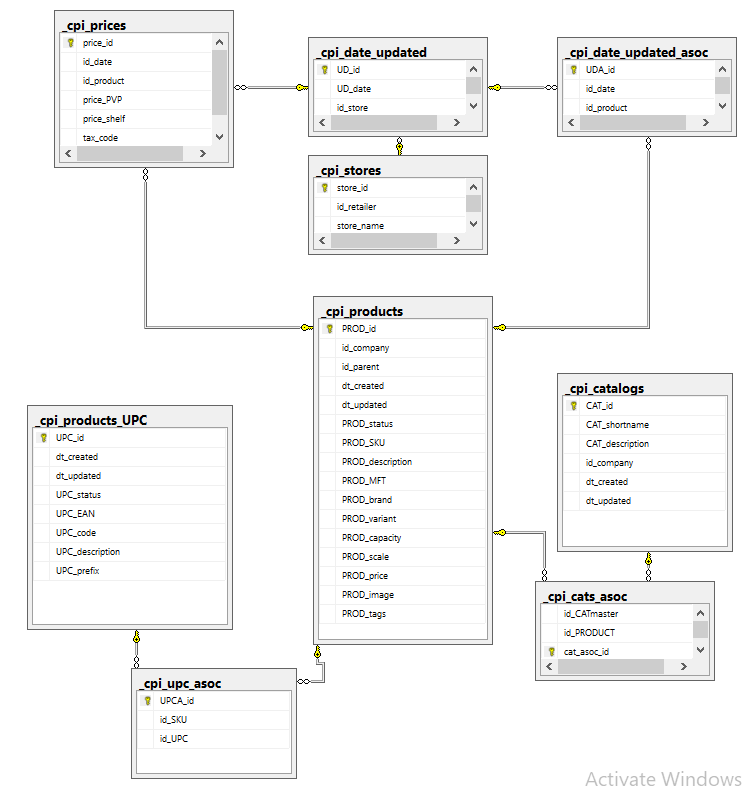
\includegraphics[width=\textwidth]{er.png}
       \caption{Diagrama ER}
       \label{fig:er}
       \centering
 \end{figure}